\documentclass[UKenglish]{article}  %% ... or USenglish or norsk or nynorsk
\usepackage[utf8]{inputenc}           %% ... or latin1 or applemac
\usepackage[T1]{fontenc,url}

\usepackage[a4paper]{geometry}
\usepackage{listings}

\setlength{\parskip}{1em}
\setlength{\parindent}{0em}
\usepackage{caption}
\usepackage{subcaption}


\urlstyle{sf}
\usepackage{tikz,babel,textcomp,csquotes,pgf-umlsd,varioref,graphicx, float}
\usepackage{array}
\usepackage[font={small,it,sf}]{caption}
\usepackage{longtable}
\usetikzlibrary{arrows, shadows}
\title{Project 1}        %% ... or whatever
         %% ... if any
\author{Aulon Mujaj, Henning Lund-Hanssen, Espen Jones}                      %% ... or whoever 

\begin{document}
\maketitle{}

\section{Requirement 1 - Brief analysis}

\subsection{Brief description}
This program is a simulation of the popular game Minesweeper. In this version of
Minesweeper, the player is presented with a map of coordinates with
question marks. Under each question mark, there is either a number representing
how many mines that are in the vicinity of this particular point on the map, or,
a mine. The player is prompted for a set of coordinates, which should correlate
to a question mark on the map that the player does not think has a mine beneath
it. The game goes on for as long as the player does not hit a question mark with
a mine beneath. The game ends when the player has identified all of the
question marks without a mine, or if the player hits a question mark with a mine.

\subsection{Analysis}
We applied experience-based testing with the Minesweeper game. We have all
played it at some point and know how it should operate in order to mimic the
original game to a satisfactory grade. We have also developed several games
running in the terminal on Java. Therefore, we used experience-based testing.

Through our experience, these type of applications have got to handle several
types of erronous input from the user. This includes coordinates outside the
minefield and text commands that the system does not recognize. No command
should crash the program or create a state that we cannot recover from, except
from the "exit" command, which should exit the program.

\subsection{Non-functional tests}
Non-functional tests should always be tested. Though, this code looks like it
was submitted in some introduction course in Java programming. If we look on
this as a mandatory assignment in such a course, the only non-functional
requirement is that it should run on every machine at UiO with Java. If this
were to be a huge game developed by a real company with the goal of making a
multiplayer Minesweeper game with a regional high score for each country and so
on, the non-functional requirements would change.

\subsubsection{Performance, load and stress}
The program should not strain the computer to the point where Minesweeper
prevents normal execution of other programs. 

\subsubsection{Reliability}
If the program crashes, it does not save the state, so it is not recoverable
after a crash. Though, the original game of Minesweeper does not do this either.

\subsubsection{Usability}
Playing the game requires the player to have previous knowledge of coordination
systems. The instructions on how to play the game is lacking to some degree. It
is a single line that instructs the user to give coordinates as input and to not
step on a mine. This is forgiving to some degree, as most players have previous
experience with the Minesweeper game.

\subsubsection{Efficiency}
The program operates instantaneously both when it comes to asking for input and
calculating the high score. Also, the program as a whole does not utilize
more resources than it needs to.

\subsubsection{Maintainability}
If changes is to be made to this system, the programmer has to know the Java
programming language. If not, it as to be written from scratch in order for a
change to be made. We all know how to program Java, so this particular
non-functional test will not be performed.

\subsubsection{Portability}
The only requirement for the program to be run is Java. The program can be run
automatically with an IDE like IntelliJ or Eclipse. Without an IDE, you have to
have some knowledge about the Java Platform. An alternative to just use the Java
compiler and platform is to use a software project management system like Maven,
Ant or Make.

\subsection{Test cases}
Test cases sorted from most important to least important.

\begin{table}[H]
    \centering
    \begin{tabular}{| m{1.5in} |  m{1.5in}  | m{1.5in} | m{0.75in} |}
        \hline

        \textbf{Pre-status} & \textbf{Test} & 
        \textbf{Expected result} & \textbf{Actual result} \\ \hline

        Program not running & Starting the program with IDE & Show the minefield
        and prompt the user for an action  & As expected \\ \hline

        Program running & Giving the program input to a coordinate without a
        mine & Show the field with a number representing adjacent mines & As
        expected \\ \hline

        Program running & Giving the program input to a coordinate with a mine &
        End the game, show the spot where the user hit a mine, the rest of the
        mines and prompt the user for a name to be used in the high score list &
        As expected \\ \hline

        Program running & Giving the program input to the text command "exit" &
        Prompt the user for a high score name, print the high score and exit &
        As expected \\ \hline

        Program running & Giving the program input to the text command "top" &
        Display the high score list & As expected \\ \hline

        Program running & Giving the program input to the text command "restart"
        & Prompt the user for a high score name and restart the game the game &
        Almost as expected - also displays the high score list \\ \hline

        Program running & Play the game 1 round, exit the program and restart
        it & Game does not remember the 1 round from before we exited & As
        expected \\ \hline

        Program not running & Launch the game, play and show off all commands &
        Understand how to play the game just by reading the instructions given
        by the program itself & As expected \\ \hline

        Program not running & Starting the program to check system resource
        usage & Should not make the computer noticeably slower during any
        operation of the system & As expected \\ \hline

        Program running not relevant & Launch the game through the command line
        with Java & Should be able to launch the game & Everyone made it - As
        expected) \\ \hline
    \end{tabular}
\end{table}

Without previous knowledge of this program, we would be forced to look more into
the code in order to understand what should be possible and what should not.
This is because the documentation of this program is seriously lacking. Our
previous knowledge of these kinds of programs also helped us to test the input
handling of the system.

\section{Requirement 2 - In-depth metrics}

\subsection{Metrics at project level}
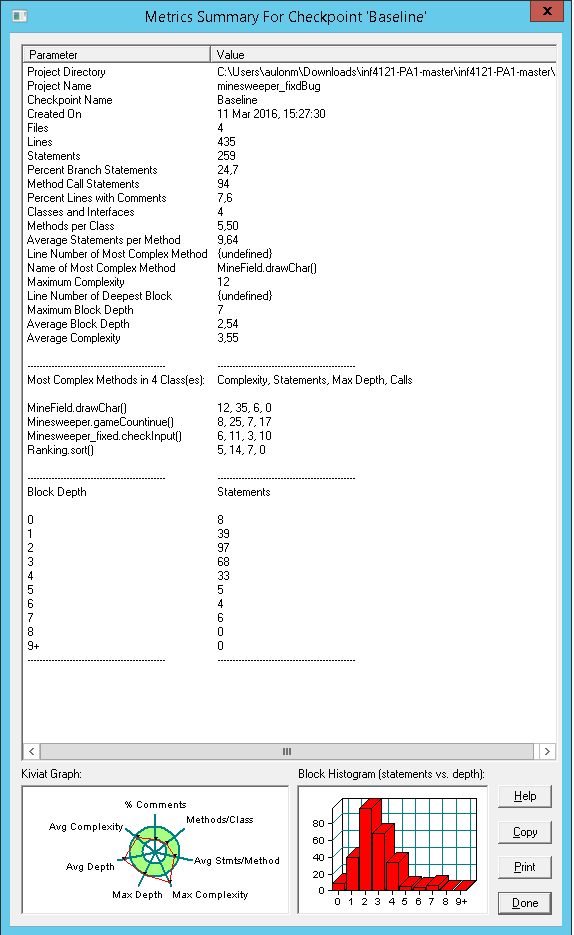
\includegraphics[height=8cm]{metric_summary}
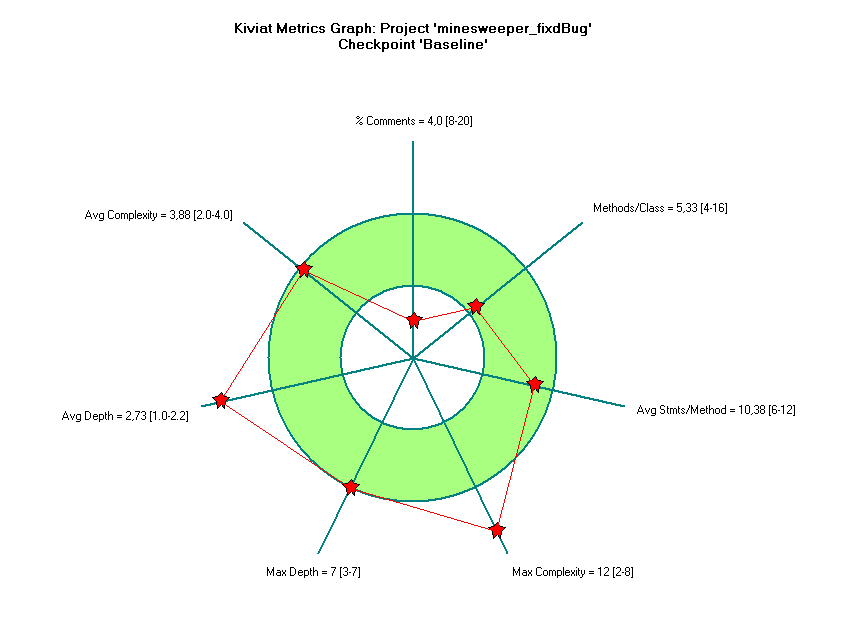
\includegraphics[height=8cm]{kiviat_diagram_baseline}
We used SourceMonitor to check which file was the biggest in our project by the number of lines in code. At the same time we needed to find the file with most branches and most complex code. On all three occurrences, it was MineField.java that had the most complex code, most lines and most branches. We could see from the kiviat graph that because of the depth at 6, the max complexity at 12 and average depth at 2.7, that the code from MineField is the most complex code of all of them. 

\begin{longtable}[H]{| m{1in} |  m{2in} | m{2in} |}
       \hline
       \textbf{Metric} & \textbf{Description} & \textbf{Explanation}\\
       \hline
        Files & How many files the project has in total & Our project has three files\\
       \hline
       Lines & Total lines of code throughout the project & There are a total of 325 lines in our project\\
       \hline
       Statements & Statements are lines that are terminated with a semicolon character. Branches such as if, for, while are also counted as statements, so are control statements try, catch, finally and throw. & 198 statements\\
       \hline
       Percent Branch Statements & The percent branch statements is how much percent of all the statemtns are branch statements in our project. & From the total of 198 statements, are only 27.3\% of those branch statements\\
       \hline
       Method call statements & All calls are counted, both in statements and in logical expressions. & There are 64 method call statements\\
       \hline
       Percent lines with comments & Off all the lines throughout the project, how many of those lines are comments. &  Only 4\% of the lines are comments. This is a little low, since we would like to have them between 8-20 percent. If the code is complex, then it needs comments, while easy to understand code does not necessarily need comments. This needs to change when we refactor \\
       \hline
       Classes and Interfaces & SourceMonitor checks for the name ``class <class name>'' or ``interface <interface name>'' and extracts the calss names. Both interfaces and classes are counted together. & Three classes and no interfaces \\
       \hline
       Methods per class & Total method count divided by the total class count & 5.33 methods per class, and it is expected to be between 4-16, which it is. Does not really need to change that much, but a few more methods would benefit the whole project. It's important that a method does not have too many statements. Better with methods with few statements, than the other way\\
       \hline
       Average Statements per Method & Total number of statements found inside of methods divided by methods found in the file. & Average statements per methods is 10.38, which means to us that it is on the border of going over exptected. We should refactor the code in a way that each method has less statements, but there are more methods \\
       \hline
       Name of most complex methods & The method that is the most complex one & MineField.drawChar()\\
       \hline
       Maximum Complexity & Count of the number of basic decision in a function assigning 1 point to each of the following: the function, each if, while, switch, case, for statements and each || or \&\& within a conditional & Our project has a maximum complexity of 12, which is too high and over exptected. We would like to have it down to between 2-8. \\
       \hline
       Maximum Block Depth & Start of each file is level zero, each indent is one depth & Our project has a maximum block depth at 7, which is over what we would like to have. It would be better if it was at a maximum of 3 depths, and need to change a few of the for loops and if statements \\
       \hline
       Average Block Depth & Weighted average of the block depth of all statements of the project & The average depth is 2.73, we would like to ahve it at 2.2 at the highest. When we change the maximum block depth part, then this one will also change accordingly \\
       \hline
       Average Complexity & Measure of the overall complexity for each method in a file or checkpoint. & Average complexity is 3.88. Here we need to change how many statements and conditionals we use, the less the better. We would like to have it at most at 3.\\
       \hline
       Most complex methods & Shows the most complex methods of the whole project, and shows the different numbers for complexity, statements, max depth and calls that it does. & MineField.drawChar(), MineSweeper.gameContinue() and Ranking.sort() are the msot complex methods in three classes. We are going to change the MineSweeper class, where complex, stmts, dept and calls are 8,25,7,0. We are going to change that to a much lower number on each, hopefully 3 in depth, which is the most important one\\ 
       \hline
       Statements on each block depth & Shows how many statements each block depth has & - We see from the summary that there are too many statements from depth 4 to 7. We are going to get rid of most of them, and have the most statements on depth 2, at most 3. \\
       \hline
\end{longtable}
\subsection{Metrics at file level}
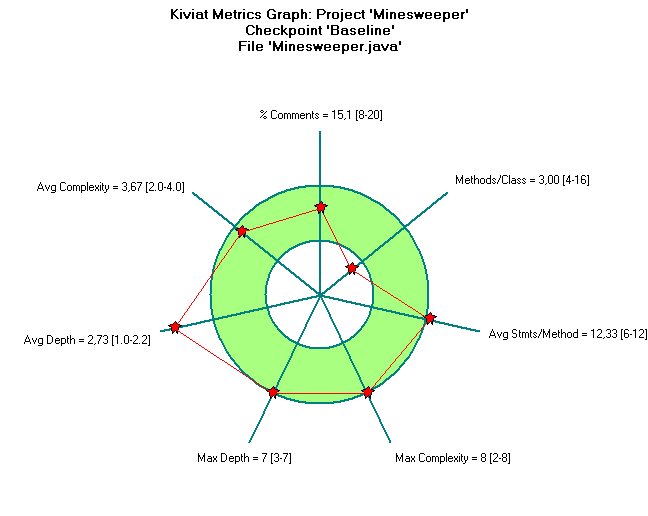
\includegraphics[height=8cm]{kiviat_diagram_minesweeper}

We decided to check the metrict of minesweeper.java file. Here we can see that the average complexity is at about 3.67, while the whole project is at 3.88. We can conclude from this that they are at the same point on the metric scale, but it is still a little high. What we would like to have is at about 2 on the scale. 

Average depth is the same on both the whole project and in the specified file. The depth is too high and we should refactor it so that it goes down to about 1-2.2. 

Max depth is at about 7, which we find is too high and we want refactor it to about 2-4, it is the same for the whole project. If the max depth starts to be higher than 4, then the complexity of the program goes up, and that becomes a problem when you want to debug or add more functionality to the code. 

The whole project has 4\% comments in total from all the lines, while minesweeper.java is at about 15\%. This is ideal for the specific file, but not with the whole project, it should be at about the same as the specific file. On the other hand, if the code is easy to understand and does not have any complex code, then it shouldn't become a problem. 

The methods/class is at 3, when it should be between 4 and 16, while the whole project is at 5.33. Some of the methods should be divided into smaller methods, to spread the different functions of the overall code. It will be easier to understand the code, then have everything in one method.

The average statements/method is why we should refactor the code into more methods, because then the average statements/method is lower. At the moment it is at about 12.33, while the project is at 10.38, and we would like to have it between 6 and 12. 

The max complexity on the whole project is at 12, which is pretty high, and on our specific file the max complexity is 8, which is also high. We should refactor the code, so that the complexity is under 8, hopefully at 4. 


\begin{itemize}
\item Would you refactor (re-write) any of the methods you have in this file?
\end{itemize}

\section{Requirement 3 - Code improvement}
\subsection{Identification of metrics}
For the whole project the two metrics that needs work are comments, average
depth and max complexity. 

For the file Minesweeper.java the two metrics that are outside of ... are 
'Method/class' and 'Avg. Depth'. These two metrics are pretty good correlation.
By moving code in nested if-statements or that in some way have a high depth 
into methods, this will give less 'Avg. depth' and more Methods per Class. 
But this also correlates to 'Avg.Complexity' and 'Avg. Statements per method'.
By creating a lot of methods that does only a small amount, meaning they have
low complexity and low number of statements, these two metrics would be lowered.

The code is not really documented either, but includes code disabled by being
commented out. This metrics looks fine, but after removing the disabled code,
no comments remain.

\subsection{Changes: Minesweeper.java}
First of the file Minesweeper.java has a lot of unnecessary indentations, which
give higher average depth for no use. For example this part:

\lstinputlisting[language=Java]{code_examples/indent.java}

Here we have two completely redundant indentations. Both 
'rank.recordName(result) and 'return true;', have no reason to be indented, and 
would yield the same result by being at the same depth as the print-line. 

A second code bit for improvement is the 'gameContinue()' method. This part does
a lot of work on depth four, and much of the work would be natural to insert
into sub-methods, granting cleaner code and more in-line with the kiviat
metrics. I chose to create a separate method for checking input, called from
gameContinue(), in addition all game action calls on methods to do the work,
instead of doing the work at the level four depth. 

To avoid lowering the 'Statements per method' and avg. Complexity, I've
combined methods for similar functions. The 'restart', 'exit' in addition to
trigger for game lost and game won does more or less the same, so it's clearly a
good practice to gather these code executions into one method like this: 

\lstinputlisting[language=Java]{code_examples/endRound.java}

I also changed some of the logic in the code, making it easier to split code
into methods. gameContinue() is no longer a boolean, but an int and return codes
based on the reason for game end or game game status. The 'gameContiue()' method
will return the code from checkInput unless the code is GAME\_CONTINUE.

\lstinputlisting[language=Java]{code_examples/game_codes.java}

Lastly inserting simple documentation for every method will suffice for keeping
the '\% comments' inside recommended values.

\subsection{Results from changes}
\begin{figure}[h]
	\begin{subfigure}[b]{0.5\textwidth}
		\caption{Kiviat graph of Minesweeper.java before changes}
		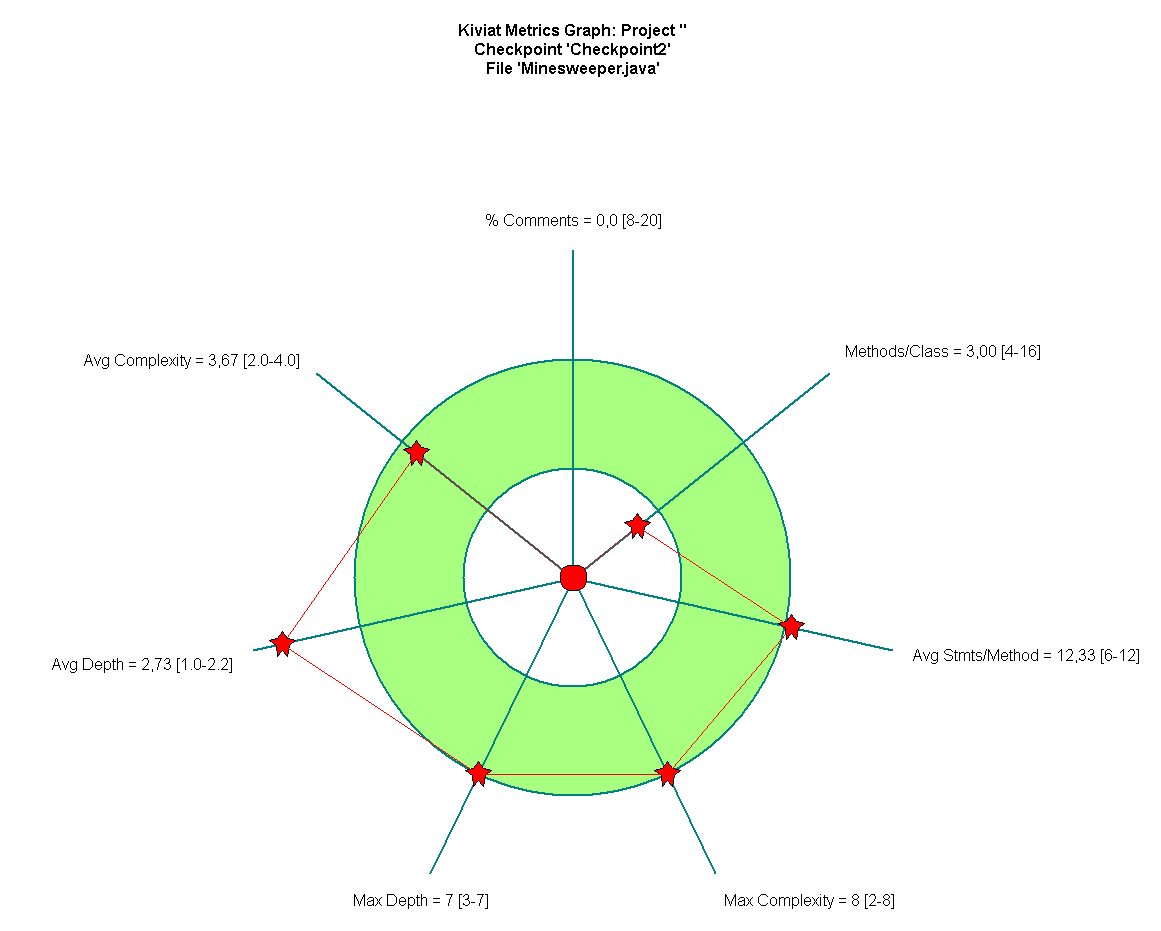
\includegraphics[width=\textwidth]{kiviat_minesweeper_before}
		\label{minesweeper_before}
	\end{subfigure}
	\begin{subfigure}[b]{0.5\textwidth}
		\caption{Kiviat graph of Minesweeper.java after changes}
		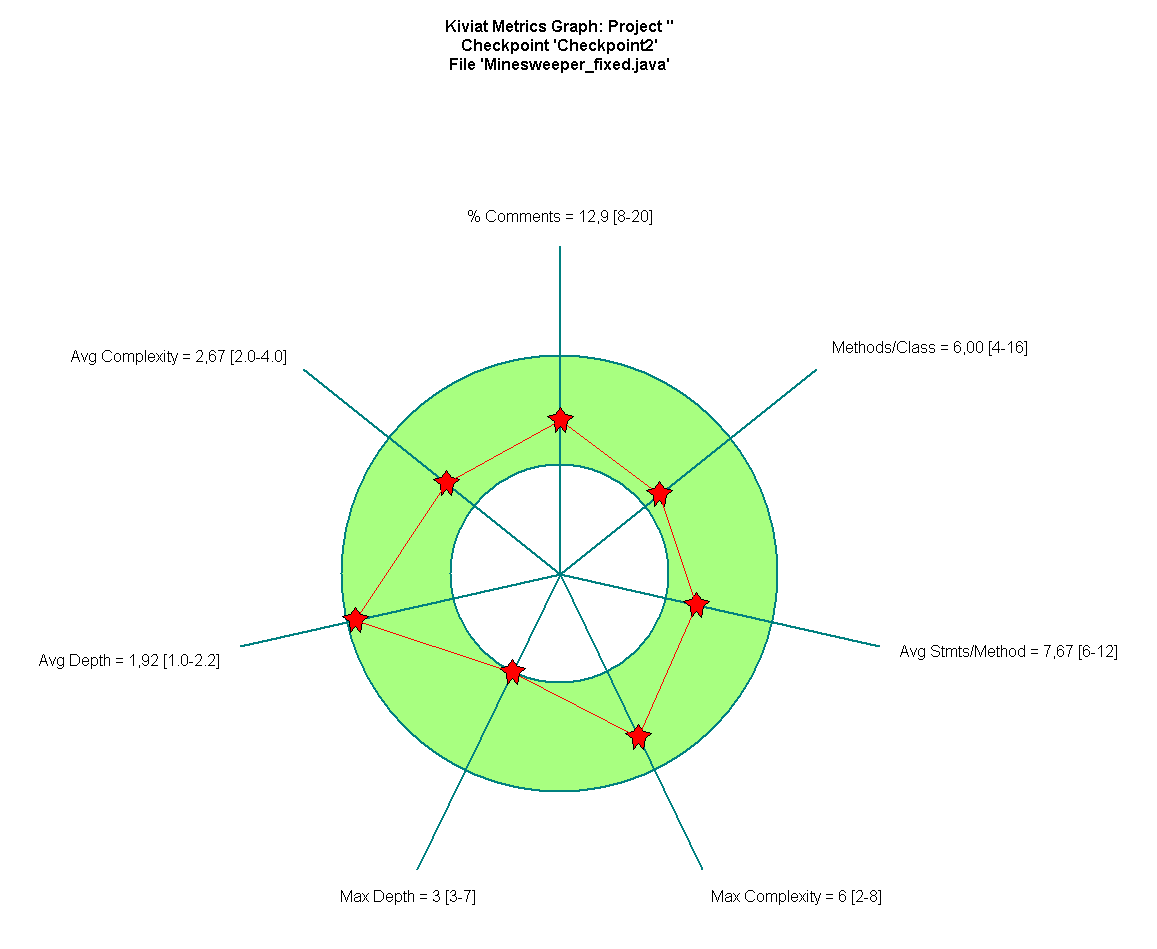
\includegraphics[width=\textwidth]{kiviat_minesweeper_after}
		\label{minesweeper_after}
	\end{subfigure}
\end{figure}

Figure \ref{minesweeper_after} Shows that the kiviat metrics are all inside 
recommended values. The intention was as mentioned to up Methods per class, and
decreasethe average depth, while keeping the rest inside recommended metrics. 
All metrics have been altered by the changed, but by the though process of the
improvement all metric are inside recommended values. The most notable change
from figure \ref{minesweeper_before} is the max depth, which is plainly is the
removal of the redundant indentations. Also the avg complexity and avg 
statements.
per method has been lowered in affect to the introduced 'helper' methods. 

\begin{figure}[h]
	\begin{subfigure}[b]{0.5\textwidth}
		\caption{Kiviat graph of the whole project before changes}
		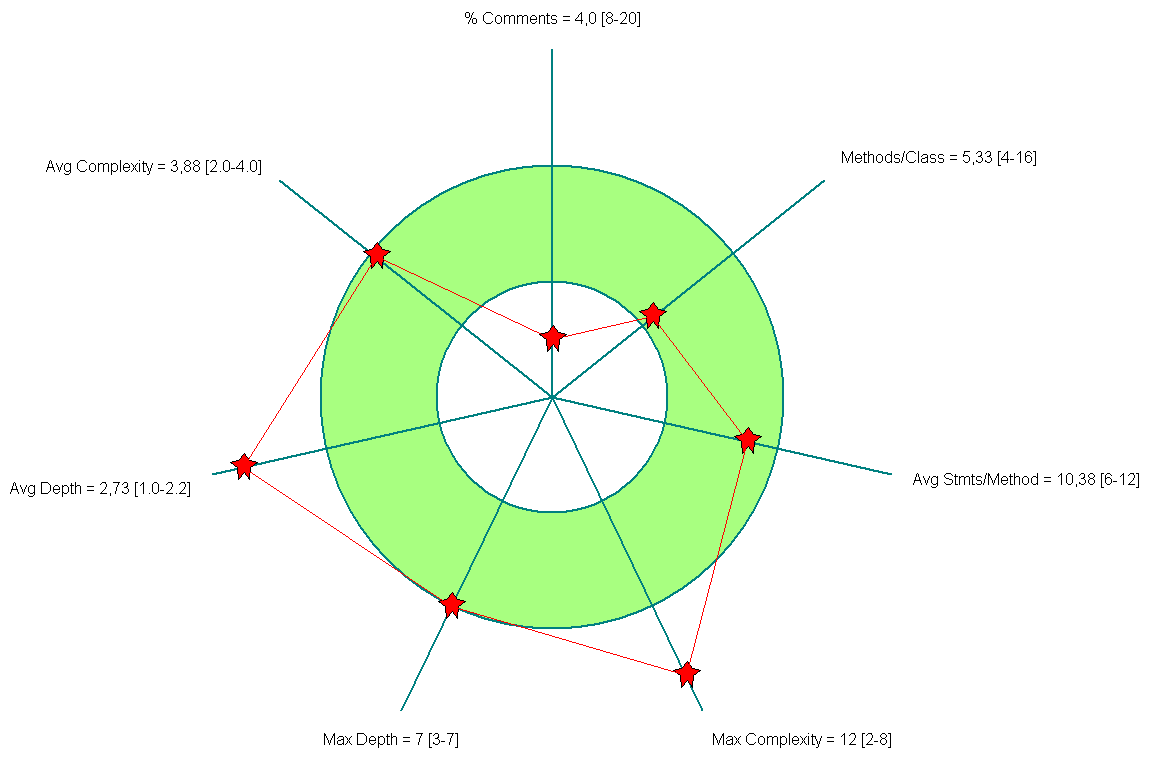
\includegraphics[width=\textwidth]{kiviat_project_baseline}
		\label{project_before}
	\end{subfigure}
	\begin{subfigure}[b]{0.5\textwidth}
		\caption{Kiviat graph of the project after changes}
		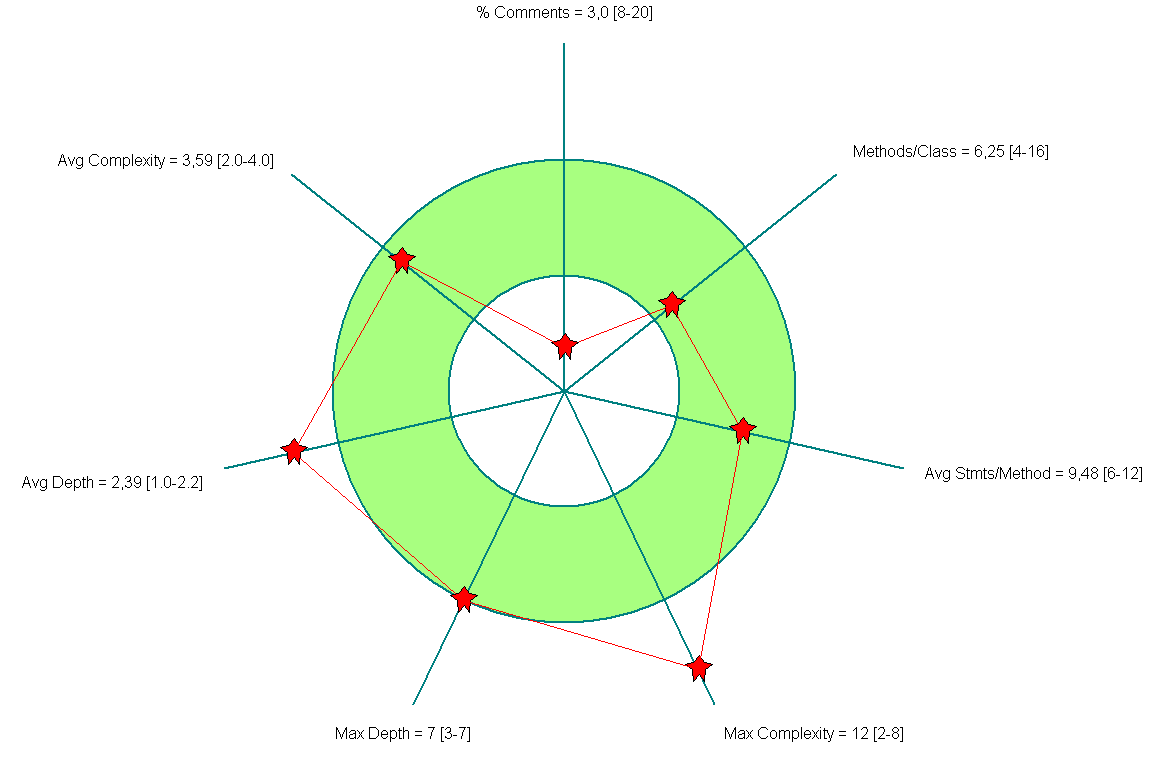
\includegraphics[width=\textwidth]{kiviat_project_after}
		\label{project_after}
	\end{subfigure}
\end{figure}


\subsection{Final remarks}
It was not so easy as it seemed to maintain the code. Almost all the values
depend on each other in some way, and by decreasing the depth by creating more
helper methods, the complexity and average complexity decreased naturally. You
could not just improve one metric without thinking about the other. But with
some planning and given there are not too many metrics to keep in mind, the
improvement went rather smoothly.
\end{document}
